\section{Phenix EMRinger protocol}
\label{app:emRingerProtocol}%a120
Protocol designed to assess the geometry of refined atomic structures regarding electron density maps in \scipion by using $EMRinger$ \citep{barad2015}. Integrated in cryo-EM validation tools of $Phenix$ software suite (\url{https://www.phenix-online.org/}) and created as an extension of the X-ray crystallography validation tool $Ringer$, $EMRinger$ tool computes the amount of rotameric angles of the structure side chains as a function of map value to assess the goodness of the fitting to the cryo-EM density map.\\

\begin{itemize}
 \item \scipion menu:\\
  \ttt{Protocols SPA -> Model building} (\ffigure{fig:app_protocol_emringer_1} (A))\\
  
 \item Protocol form parameters (\ffigure{fig:app_protocol_emringer_1} (B)):\\
  
    \begin{figure}[H]
     \centering 
     \captionsetup{width=.7\linewidth} 
     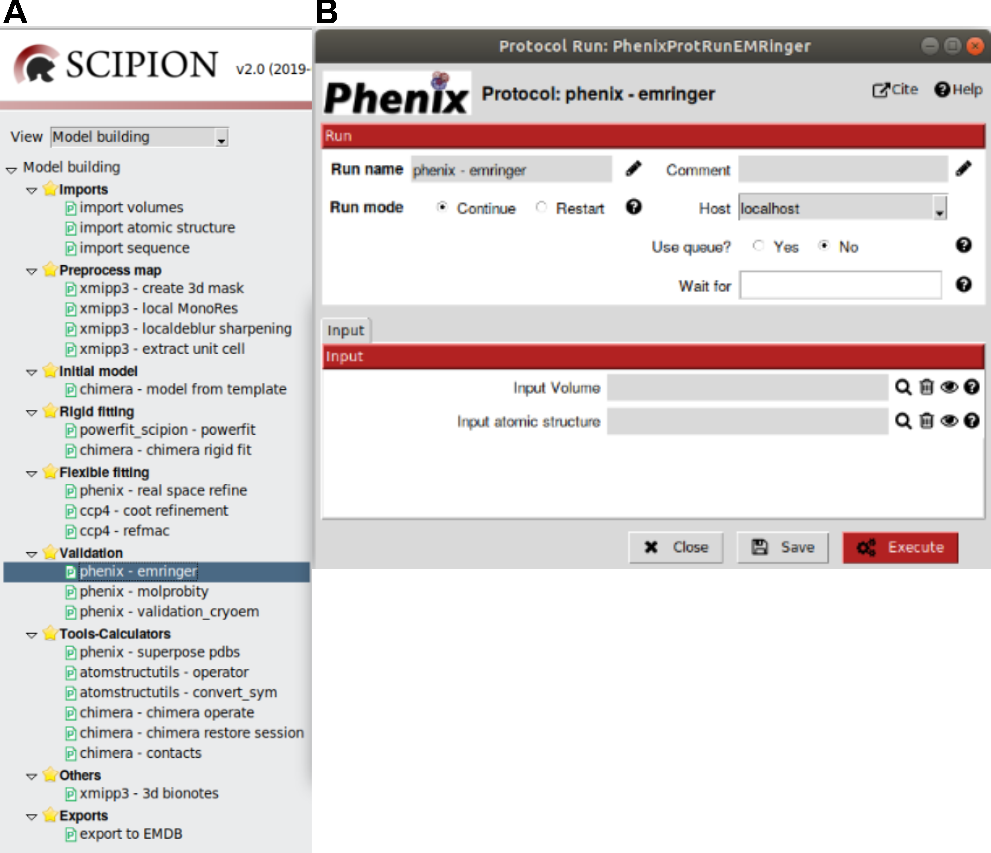
\includegraphics[width=0.90\textwidth]{Images_appendix/Fig139.pdf}
     \caption{Protocol \scommand{phenix - emringer}. A: Protocol location in \scipion menu. B: Protocol form.}
     \label{fig:app_protocol_emringer_1}
    \end{figure}

    \begin{itemize}
     \item \ttt{Input Volume}: Electron density map previously downloaded or generated in \scipion and fitted to an atomic structure.
     \item \ttt{Input atomic structure}: Atomic structure previously downloaded or generated in \scipion and fitted to an electron density map.\
    \end{itemize}
    
 \item Protocol execution:\\

  Adding specific sequence label is recommended in \ttt{Run name} section, at the form top. To add the label, open the protocol form, press the pencil symbol at the right side of \ttt{Run name} box, complete the label in the new opened window, press OK, and finally close the protocol. This label will be shown in the output summary content (see below). If you want to run again this protocol, do not forget to set to \ttt{Restart} the \ttt{Run mode}.\\
  Press the \ttt{Execute} red button at the form bottom.\\
  
 \item Visualization of protocol results:\\
  
  After executing the protocol, press \ttt{Analyze Results} and the results window will be opened (\ffigure{fig:app_protocol_emringer_2}).\\ 
  
  \begin{figure}[H]
     \centering 
     \captionsetup{width=.7\linewidth} 
     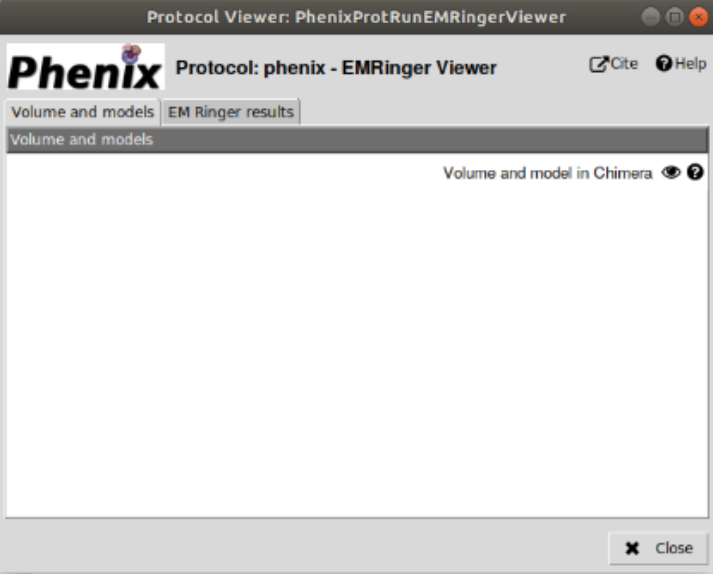
\includegraphics[width=0.60\textwidth]{Images_appendix/Fig140.pdf}
     \caption{Protocol \scommand{phenix - emringer}. Taps to visualize Volume and models or $EMRinger$ results.}
     \label{fig:app_protocol_emringer_2}
    \end{figure}
    
   Two taps are shown in the upper part of the results window:
    \begin{itemize}
     \item XXXX Maps and models:
     \chimera graphics window displays coordinate axes, selected input volume and fitted atomic structure.
     \item XXXX EMRinger Results (\ffigure{fig:app_protocol_emringer_3}):
     
     \begin{figure}[H]
     \centering 
     \captionsetup{width=.7\linewidth} 
     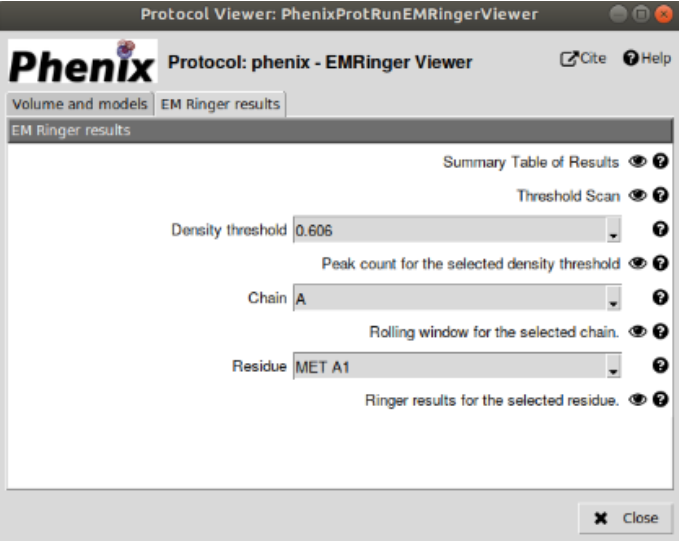
\includegraphics[width=0.60\textwidth]{Images_appendix/Fig141.pdf}
     \caption{Protocol \scommand{phenix - emringer}. Menu to visualize $EMRinger$ results.}
     \label{fig:app_protocol_emringer_3}
    \end{figure}
      \begin{itemize}
        \item XXX Results table (\ffigure{fig:app_protocol_emringer_4}):
        \begin{figure}[H]
         \centering 
         \captionsetup{width=.7\linewidth} 
         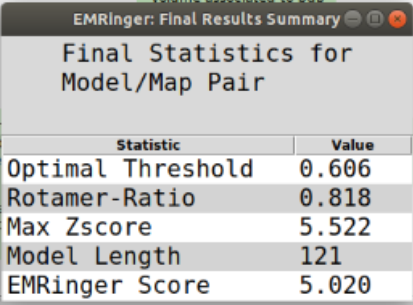
\includegraphics[width=0.60\textwidth]{Images_appendix/Fig142.pdf}
         \caption{Protocol \scommand{phenix - emringer}. Final $EMRinger$ results.}
        \label{fig:app_protocol_emringer_4}
     \end{figure}
         \begin{itemize}
          \item Optimal Threshold: Selected volume Electron Potential, in a range of 20, at which maximum values of EMRinger Score and Percentage of Rotameric Residues are reached. 
          \item Rotamer-Ratio:
          \item Max Zscore: Probability of finding a certain number of rotameric residues, at a specific side chain dihedral angle, among the total number of map peaks found above the Optimal Electron Potential Threshold, assuming a binomial distribution of rotameric residues B(\ttt{n, p)} ($n$: total number of map peaks found above the Optimal Electron Potential Threshold; $p$: 39/72; with map sampling every 5º, 39 angle binds are considered rotameric from a total of 360/5 = 72).
          \item Model Length: Total model number of residues considered in EMRinger computation, non-$\gamma$-branched, non-proline aminoacids with a non-H $\gamma$ atom.
          \item EMRinger Score: Highest Z-score, rescaled regarding model length, across the range of Electron Potential Thresholds. Since the Z-score is rescaled to the EMRinger Score according model length, EMRinger Score allows suitable comparisons among different model-map pairs. EMRinger Score of 1.0 is usual for initial models refined regarding 3.2-3.5\AA resolution maps. For high-quality models with high resolution, EMRinger Score values higher than 2 are expected.
         \end{itemize}

        \item XXX Thresholds Scan:
         \begin{itemize}
          \item Plot of EMRinger Score and Percentage of Rotameric Residues regarding Electron Potential Threshold.
         \end{itemize}
        \item XXXX
      \end{itemize}
    \end{itemize}
    
 \item Summary content:\\
 
  \ttt{SUMMARY} box:\\Statistics included in the above Final Results Table (an example can be observed in \ffigure{fig:emringer_protocol} (6):

\end{itemize}

